
%%%%%%%%%%%%%%%%%%%%%%% file typeinst.tex %%%%%%%%%%%%%%%%%%%%%%%%%
%
% This is the LaTeX source for the TDPTemplate using
% the LaTeX document class 'llncs.cls' Springer LNAI format
% used in the RoboCup Symposium submissions.
% http://www.springer.com/computer/lncs?SGWID=0-164-6-793341-0
%
% It may be used as a template for your own TDP - copy it
% to a new file with a new name and use it as the basis
% for your Team Description Paper
%
% NB: the document class 'llncs' has its own and detailed documentation, see
% ftp://ftp.springer.de/data/pubftp/pub/tex/latex/llncs/latex2e/llncsdoc.pdf
%
%%%%%%%%%%%%%%%%%%%%%%%%%%%%%%%%%%%%%%%%%%%%%%%%%%%%%%%%%%%%%%%%%%%

\documentclass[runningheads,a4paper]{llncs}
\usepackage{amssymb}
\setcounter{tocdepth}{3}
\usepackage{graphicx}
\usepackage{amssymb}
\usepackage[utf8]{inputenc}
\usepackage{url}
\usepackage{float}
\usepackage{amsmath}
\usepackage{graphicx}
\usepackage{wrapfig}
\usepackage{verbatim}
\usepackage{caption}
\usepackage{subcaption}
\captionsetup{compatibility=false}

\usepackage{lipsum}
\newcommand{\BnL}[1][1em]{ 
\includegraphics[width=#1]{images/bnl.jpg} }

\begin{document}

\title{UT Austin Villa\\ RoboCup@Home\\ Domestic Standard Platform League \\Team Description Paper}
\titlerunning{UT Austin Villa\\ RoboCup@Home\\ DSPL TDP}

\author{Justin W. Hart\and Peter Stone\and Andrea Thomaz\and Scott Niekum}
\institute{Department of Computer Science\\ Department of Electrical and Computer Engineering\\ University of Texas at Austin\\
\texttt{http://www.cs.utexas.edu/~AustinVilla/athome/Team2017/}}
\maketitle


%%%%%%%%%%%%%%%%%%%%%%%%%%%%%%%%%%%%%%%%%%%%%%%%%%%%%%%%%%%%%%%%%%%%%%%%%%%%%%%%%%%%

\begin{abstract}
Our general approach to the RoboCup@Home competition is one of integrating the HSR into the existing robotics research infrastructure of three collaborating laboratories here at the University of Texas at Austin. These laboratories focus on research toward the development of artificial intelligence, machine learning, and human-robot interaction technologies which provide services to and interact with human users in both a simulated home environment and in a live deployment known as the Building-Wide Intelligence (BWI) Project in the Gates-Dell Computer Science Complex at the University of Texas at Austin. By incorporating the HSR into our existing ecosystem, we will be able to rapidly deploy relevant components from our ongoing research into its software infrastructure for the competition. Incorporation into our existing research also guarantees the reusability of software developed for the competition as it is integrated into the large software deployment of the BWI Project. Significant portions of the code developed by our group for competition will be released as components of the BWI infrastructure code as open source software through ROS.org. Relevant current work by our groups involves research in natural language processing, multimodal language learning, learning from demonstration, human activity recognition, planning, and probabilistic and symbolic reasoning. In the past year, significant work has been performed on domestic tasks such as storing groceries, and language tasks such as natural language processing and the performance of natural language tasks from speech.

%In your abstract, please state your main research line and your achievements of this year (on which problem or set of problems are you focusing all the team efforts). Tell why this research is important, how are you approaching to the problem solution and which results do you expect to obtain.

\end{abstract}


%%%%%%%%%%%%%%%%%%%%%%%%%%%%%%%%%%%%%%%%%%%%%%%%%%%%%%%%%%%%%%%%%%%%%%%%%%%%%%%%%%%%

\section{Introduction}
The UT Austin Villa team, from the University of Texas at Austin, has a long and successful history of RoboCup participation. In 2016, we finished 2nd place in the soccer standard platform league (SPL), and won first place in the 3D simulation league for the 5th time in 6 years.  Although we have also pursued research on domestic and service robots for many years, we have only once participated in RoboCup@Home, finishing in 2nd place in 2007.  This application brings together the laboratories of UT Austin Villa founder and team leader of Prof. Peter Stone with those of two colleagues at UT Austin who are experts in interactive robotics, but who have never participated in RoboCup: Prof. Andrea Thomaz and Prof. Scott Niekum. Our entry in the 2017 RoboCup@Home competition will unite these three groups to focus our complementary research in the areas of machine learning, service robotics, and human robot interaction towards an entry in the RoboCup@Home SPL using the Toyota Human Support Robot (HSR).

\section{Approach}
The laboratories of Stone, Thomaz, and Niekum currently have active research programs that are directly relevant to the challenge put forth by the RoboCup@Home competition. Prof. Stone's laboratory is pursuing the Building-Wide Intelligence (BWI) project, which includes a group of several human-interactive robots, and which has the long-term objective of enabling a team of robots to achieve long-term autonomy within the rich socially interactive environment of the UT Austin Computer Science Department in the Gates-Dell Complex. Profs. Thomaz and Niekum have performed much of their past research in home-like environments and have an existing shared lab space set up as an apartment with a living room, dining room, and kitchen. Currently, our groups use similar, but distinct robot platforms. The BWI project uses a fleet of SegBots, Figure \ref{fig:1a}, custom designed mobile robots built atop Segway RMP bases. In the past year BWI has been performing robot learning experiments with a SegBot with Kinova Mico arm mounted, Figure \ref{fig:1b}. Thomaz and Niekum use a pair of similar custom robots atop an omni-drive base, both with arms, Figure \ref{fig:1c}. The basic approach that our team will take in the RoboCup@Home competition is to integrate the HSR platform into the fleet of robots used in the Building-Wide Intelligence project, and to use development on the shared common platform of the Toyota HSR towards the RoboCup@Home competition as a means of integrating research across our laboratories.

\begin{figure}	
	\centering
	\begin{subfigure}[t]{1.4in}
		\centering
        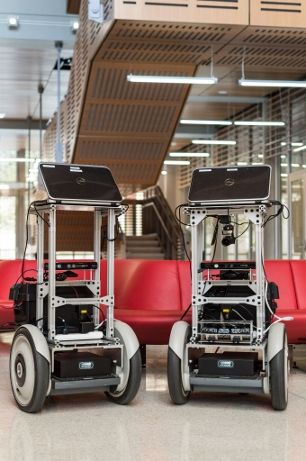
\includegraphics[width=\textwidth]{images/bwi1.jpg}
		\caption{Two SegBots from the Building-Wide Intelligence Project at UT Austin.}\label{fig:1a}		
	\end{subfigure}
	\quad
	\begin{subfigure}[t]{1.4in}
		\centering
        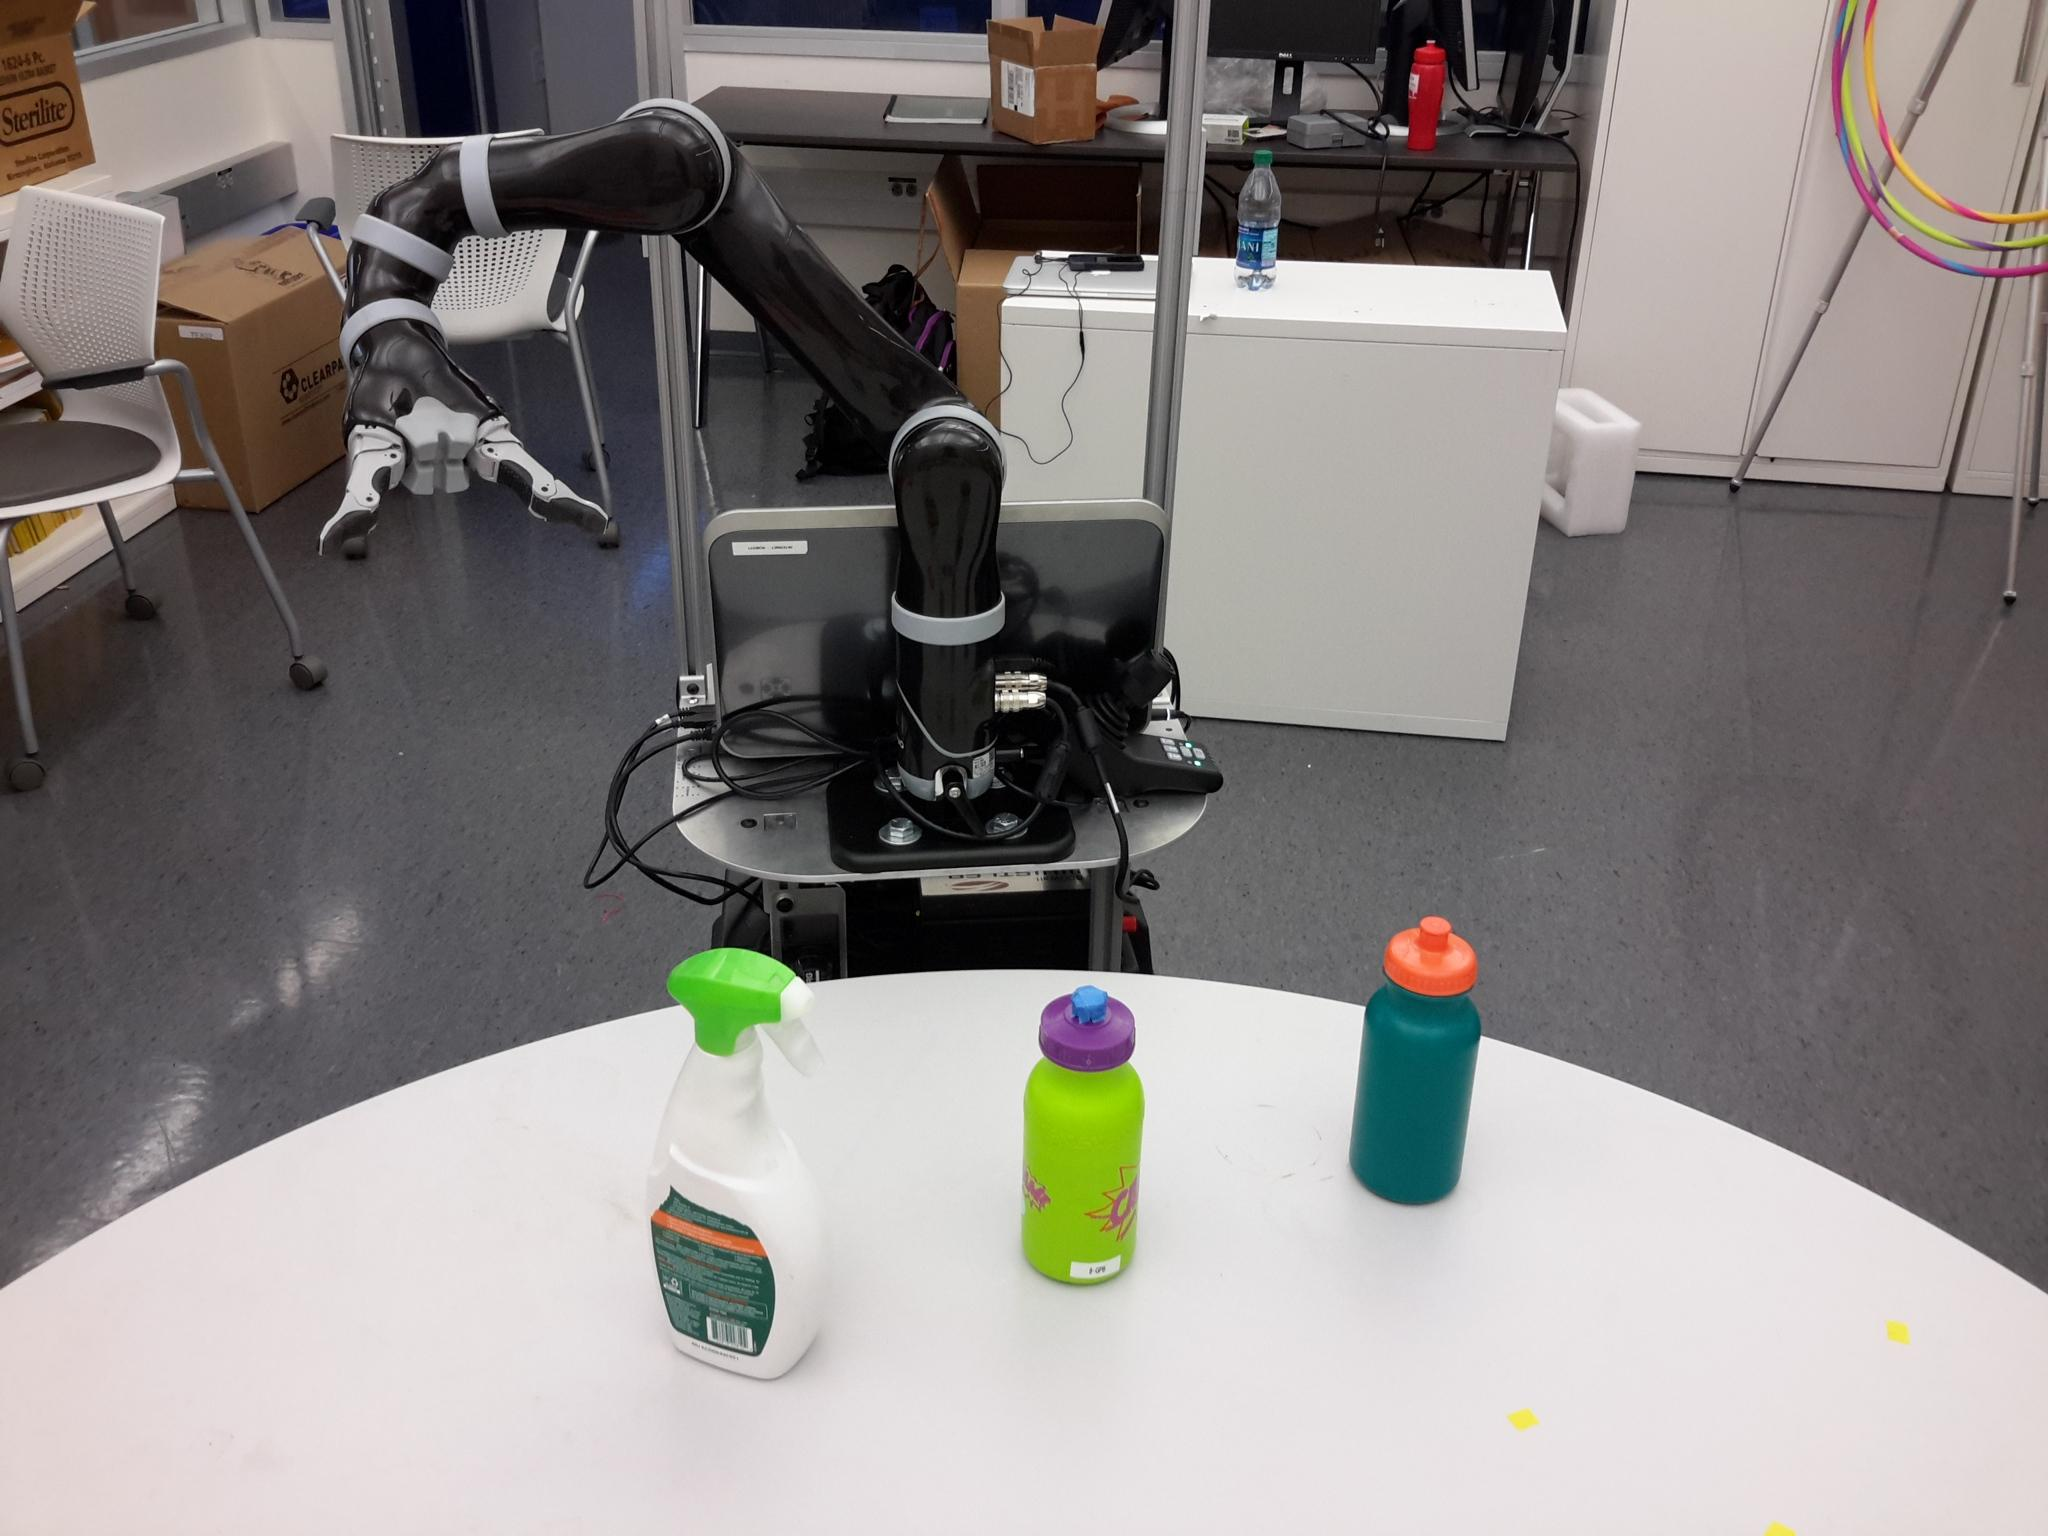
\includegraphics[width=\textwidth]{images/bwi_arm.jpg}
		\caption{SegBot with mounted Kinova Mico arm.}\label{fig:1b}
	\end{subfigure}
	\quad
	\begin{subfigure}[t]{1.4in}
		\centering
        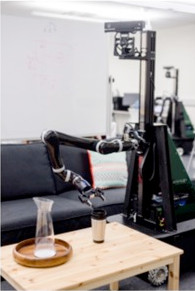
\includegraphics[width=\textwidth]{images/ut_poli.jpg}
		\caption{Custom robot used in the simulated home environment in Thomaz and Niekum's shared laboratory space.}\label{fig:1c}
	\end{subfigure}
	\caption{Robotic platforms currently in use in research by members of the UT Austin Villa RoboCup@Home Team. These platforms are similar to the Toyota Human Support Robot (HSR), which will be used in the Domestic Standard Platform League competition.}\label{fig:1}
\end{figure}

Among the central goals of our research is the development of robotic systems capable of long-term autonomous human-robot interaction, automated planning, reasoning, and learning in complex real-world environments. By defining a novel competition framework situated within a domestic environment that uniquely exposes the challenges of this proposition, RoboCup@Home is an ideal setting for advancing the state of the art in long-term autonomy for human-interactive robots, and presents a both a task framework that is harmonized with our goals and a standard set of tasks against which we can compare our platform to other systems. With this motivation in mind, it is our goal to combine the expertise of Profs. Stone, Thomaz, and Niekum in the areas of reinforcement learning, human-robot interaction, and learning from demonstration towards a full solution to the RoboCup@Home challenge, along with their laboratories. Our team brings together postdocs, graduate students, and undergraduate students from each of our groups to enable the robot to interact seemlessly with people in the environment, and to learn behaviors ranging from object manipulation to robust environmental perception, to high-level task sequencing.

By leveraging our existing software and incorporating our HSR into the BWI infrastructure, we hope to gain a jump start on the competition. We will also be able to make use of the infrastructure which we have in place for experiments on human-robot interaction in domestic and public spaces. Thomaz and Niekum's shared laboratory space is located in the same building as the BWI project, allowing us to test our system in both an open, interactive setting with many people to potentially interact with, and more controlled home-like settings. We expect that participation in the RoboCup@Home will boost our research efforts through collaboration between our groups, the sharing of ideas in an environment of friendly competition, and the advancements required to accomplish the tasks of the competition itself. We expect to make advancements on topics ranging from activity recognition, to robust perception, to learned planning and navigation, to general human-robot interaction.

%\section{Externally Available Components}

%Upon receiving the HSR robots, we will be able to ramp up quickly by building upon the extensive ROS ecosystem and other externally available software, as well as upon our existing BWI software infrastructure and our home-robotics research.

%Our own contributions to the growing ecosystem of externally available components, including a general architecture for service robots, robot reinforcement learning software, robot learning from demonstration software, and a package for tag-based perception are listed in Section~\ref{sec:reuse} below, with links on the application webpage.

\section{Research Focus}

Our main research foci from a technical perspective are on
reinforcement learning, especially as applied to real robots,
multi-robot systems, human-robot interaction, and learning from
demonstration.  However we also have a strong history of creating
integrated, fully autonomous systems with the idea that integration is
an important and valuable research focus in and of itself.  We view
RoboCup@Home as a perfect setting for both stretching our core
research competencies and for supporting our commitment to
integration.

Examples of our past research innovations related to RoboCup@Home are
provided in Section~\ref{sec:tech}.

\section{Innovative Technology}
\label{sec:tech}

The collective breadth of our research has enabled contributions to a
variety of AI sub-areas beyond HRI, including AI planning, knowledge
representation and reasoning, natural language processing, and machine
learning.  Here we provide a brief description of some of our
published research, some of which will form the core of our
RoboCup@Home approach, and some of which we expect to be substantially
extended and improved through our participation in RoboCup@Home.

\begin{description}

\item [Understanding natural language requests:] 
One of the most natural forms of human-robot interaction for humans is through natural language.
However natural language processing remains a challenging research area within AI, and intelligent service robots should be able to efficiently and accurately understand commands from human users speaking in natural language.

We introduced research contributions pertaining to language learning
to facilitate on-line improvement of the robots' understanding of
spoken commands.  We use a dialog agent embodied in a BWIBot to
communicate with users through natural language and improve language
understanding over time using data from these conversations
\cite{thomason:15}.  By learning from conversations, our approach can
recognize more complex language than keyword-based approaches without
needing the large-scale, hand-annotated training data associated with
complex language understanding tasks~\cite{thomason:15}. 

To this end, we trained a semantic parser with a tiny set of
expressions paired with robot goals.  The natural language
understanding component of our system is this semantic parser together
with a conversational dialog agent.  The dialog agent keeps track of
the system's partial understanding of the goal the user is trying to
convey and asks clarification questions to refine that understanding.

%\item[Understanding natural language requests:] Since one of the most
% convenient means for humans to convey instructions is natural
%language, we have introduced methods enabling natural language
%requests to be understood by robots by grounding requests using a
%robot's existing domain knowledge, and how robots can incrementally
%learn larger vocabularies through conversation~\cite{thomason:15}.

\item[Grounded multimodal language learning:] Often it is necessary
for a robot to ground language using its own perception and actions
with respect to objects.  Consider the case where a human asks a
service robot, ``Please bring me the full red bottle''.  To fulfill
such a request, a robot would need to detect objects in its
environment and determine whether the words ``full'', ``red'', and
``bottle'' match a particular object detection.  Furthermore, such a
task cannot be solved using static visual object recognition methods
as detecting whether an object is full or empty may often require the
robot to perform a certain action on it (e.g., lift the object to
measure the force it exerts on the arm).

This research contribution~\cite{thomason:ijcai16} focused on solving the {\it symbol
grounding problem} \cite{harnad1990symbol}, a longstanding challenge
in AI, where language is grounded using the robot's perception and
action.
%~\cite{tellex:ai11,matuszek:icml12,krishnamurthy:acl13,perera:aaai13,kollar:rss13,tellex:rss14,matuszek:aaai14,parde:ijcai15,spranger:ijcai15}.  
To address this problem, we enable a robot to undergo two distinct developmental stages:

\begin{enumerate}
\item {\it Object Exploration Stage} -- the robot interacts with objects using a set of exploratory behaviors designed to produce different kinds of multi-modal feedback.
\item {\it Social Learning Stage} -- the robot interacts with humans in order to learn mappings from its sensorimotor experience with objects to words that can be used to described the objects.
\end{enumerate}

%\item[Grounded multimodal language learning:] We have introduced
%algorithms enabling a robot to learn to ground certain human
%instructions, such as ``Bring me a full, red bottle.'', in its
%perception and actions~\cite{thomason:ijcai16}.

\item[Learning multi-step tasks from demonstration:]
Much previous research in learning from demonstration has focused on
learning policies---mappings from states to actions---for skills such
as a tennis swing or humanoid walking.  However, these techniques
typically perform poorly for complex, multi-step tasks that cannot be
represented monolithically with a single policy.  We developed a
series of LfD algorithms that, for the first time, allowed a robot to
learn the structure of complex tasks such as IKEA furniture assembly
from a small number of
demonstrations~\cite{niekum2013semantically,niekum2013incremental,niekum2015online,niekum2012learning,niekum2015learning}. This
research led to state-of-the-art Bayesian nonparametric and control
techniques that were able to automatically identify an appropriate
number of skills from task demonstrations~\cite{niekum2012learning},
infer the goals of each
skill~\cite{niekum2011clustering,niekum2015online}, construct
controllers to accomplish these goals, and intelligently sequence
these controllers based on perceptual
feedback~\cite{niekum2013semantically,niekum2013incremental,niekum2015learning}.

\item[Robot-centric human activity recognition:] 
For a robot to effectively function in a human-inhabited environment,
it would be useful for it to be aware of the activities and
intentions of humans around it based on its own observations. For
example, consider the case where a robot is navigating a crowded
environment such as an undergraduate computer lab. If the robot could
recognize when a person needs help, or when a person is trying to
approach or engage it (or avoid it), its social and navigational
skills would improve dramatically.  For this purpose, we contributed a novel 
approach which explores how human activity can be
recognized, making it possible for a robot to understand the intent
of humans in its vicinity.

%To address visual activity recognition, the computer vision research
%community has produced a wide array of methods for recognizing human
%activities (see \cite{aggarwal2011human} for a review). Most relevant
%to our work are studies in which the video is captured by a
%robot. Such studies are relatively new and include the works of
%\cite{ryoo2015robot,lu15,ryoo13,chrungoo2014activity}. This existing
%work is subject to several limitations: 1)~The activities were not
%carried out spontaneously but rather, were rehearsed or commanded by
%the experimenters; 2)~The activities were performed by a small number
%of people, typically 5-8; 3)~The robot was typically either stationary
%or teleoperated.

%Our work on activity recognition overcomes these limitations in
%several important ways. First,
Our robot uses its autonomous
navigation capability in a large, unstructured, and human-inhabited
environment.
%, as opposed to a laboratory.  Second, 
The activities
learned by our robot were performed spontaneously by many different
people who interacted with (or were observed by) the robot, as opposed
to the standard methodology of asking study participants to perform
certain actions. 
%And third, 
In contrast to classic computer vision
approaches, our system uses both visual and non-visual cues when
recognizing the activities of humans that it interacts with~\cite{gori2015robot}.


%\item[Robot-centric human activity recognition:] We have demonstrated
%that a robot can categorize human activity more effectively when it is
%aware of its location in the environmnet in order to better understand
%the behavior of humans in its vicinity~\cite{gori2015robot}.


\item[Planning using action language ${\cal BC}$:] 
General purpose planning domain descriptions can be written using
various modes. Action languages such as ${\cal BC}$ are attractive in
task planning for mobile robots because they solve the \emph{frame
problem}, which states that many axioms are necessary to express that
things in the environment do not change arbitrarily~\cite{mcc69}.
For example, when a robot picks up an object from the table, it does
not change the location of a different object on the table.  ${\cal
BC}$ solves this problem by easily expressing rules of inertia.  In
addition, ${\cal BC}$ can solve the \emph{ramification problem}, which
is concerned with the indirect consequences of an
action~\cite{fin86}.  For example, when a robot picks up a tray from
the table, it indirectly changes the location of any object on the
tray.  ${\cal BC}$ can also easily express indirect and recursive
effects of actions.

%Existing tools such as \textsc{coala}~\cite{geb10} and
%\textsc{cplus2asp}~\cite{bab13} allow us to translate ${\cal BC}$
%action descriptions into logic programs under answer set
%semantics~\cite{gel88,gel91b}, and planning can be accomplished using
%computational methods of ASP~\cite{mar99,nie99}.

We have demonstrated how action language ${\cal BC}$ can be used for
robot task planning in domains requiring planning in the presence of
missing information and indirect/recursive action
effects~\cite{khandelwal2014planning}. While we demonstrate using
${\cal BC}$ to express a mail collection task, the overall methodology
is applicable to any other planning domains that require: recursive
and indirect action effects, defeasible reasoning, and acquiring
previously unknown knowledge through human-robot interaction. In
addition, we also demonstrated how answer set planning under action
costs \cite{eiter2003answer} can be applied to robot task planning in
conjunction with ${\cal BC}$~\cite{khandelwal2014planning}.

%\item We have demonstrated that domain knowledge and planning
%descriptions for robots can be written using action language ${\cal
%BC}$, allowing robots to achieve complex goals using defeasible
%reasoning\footnote{Defeasible reasoning allows a planner to draw
%tentative conclusions which can be retracted based on further
%evidence.} and indirect/recursively defined fluents

\item[Integrating probabilistic and symbolic reasoning:] While action
language ${\cal BC}$ can express defeasible reasoning, it cannot
express probabilities, and consequently cannot be used for stochastic
planning.  We therefore introduced a method for robots to efficiently
and robustly fulfill service requests in human-inhabited environments
by simultaneously reasoning about commonsense knowledge expressed
using defeasible reasoning and computing plans under
uncertainty~\cite{zhang2015corpp}.  We illustrated this planning
paradigm using a Spoken Dialog System (\textsc{sds}), where the robot
identifies a spoken shopping request from the user in the presence of
noise and/or incomplete instructions.  The goal of the system is to
identify the shopping request as quickly as possible while minimizing
the cost of asking questions.  Once confirmed, the robot attempts to
deliver the item.  While this planning paradigm is described in the
context of an \textsc{sds}, it can just as easily be applied to other
stochastic planning problems as well.

%Commonsense knowledge is the knowledge that is \emph{normally} true
%but not always, e.g., office doors are closed during holidays and
%people prefer coffee in the mornings.  Logical commonsense knowledge
%needs to be expressed via defeasible reasoning, and probabilistic
%commonsense knowledge needs to be expressed via probability
%distributions. In parallel with commonsense reasoning, robots
%frequently need to compute a plan including more than one action to
%accomplish tasks that cannot be completed through single actions. To
%do so, it is necessary to model the uncertainty in the robot's local,
%unreliable observations and nondeterministic action outcomes while
%planning toward maximizing long-term reward.
%
%With this motivation in mind, we introduced the \textsc{corpp}
%(COmmonsense Reasoning and Probabilistic Planning)
%algorithm~\cite{zhang2015corpp}.  While commonsense reasoning and
%planning under uncertainty have been studied separately,
%\textsc{corpp}, for the first time, exploits their complementary
%features by integrating \textsc{pomdp}s and
%\textsc{p-log}~\cite{baral2009probabilistic} and enables robots to
%simultaneously reason about both logical and probabilistic commonsense
%knowledge and plan toward maximizing long-term reward under
%uncertainty~\cite{zhang2015corpp}.

%\item We have demonstrated that robots can incorporate probability
%distributions with symbolic reasoning to implement a spoken dialog
%system, allowing them to intelligently ask questions in order to
%quickly understand human instructions~\cite{zhang2015corpp}.



\end{description}

A much more extensive list of relevant research contributions, as well
as links to our papers, is available from the application webpage.

\section{Re-Usability}
\label{sec:reuse}

Throughout our development, we will continue our strong tradition of releasing well-documented, self-contained behavior modules for components of autonomous robots that can be used by other research groups to enhance their own research.  As listed with links on the propoosal webpage, these include:

\begin{itemize}

\item Our BWI code repository provides an open source suite of ROS
packages, fully integrated into an architecture for service robots
that operate in dynamic and unstructured human-inhabited environments.
It has been built on top of the Robot Operating System (ROS)
middleware framework~\cite{quigley2009ros}, and is available
open-source at \url{https://github.com/utexas-bwi/}. This software
architecture provides a hierarchical layered approach for controlling
autonomous robots, where layers in the hierarchy provide different
granularities of control.  Specifically, this architecture includes
navigation software that allows a mobile robot to move autonomous
inside a building, while being able to switch 2D navigational maps
when using the elevator to move to a different floor. A symbolic
navigation module is built on top of this autonomous navigation module
which allows the robot to navigate to prespecified doors, rooms, and
objects in the environment.  From a high-level perspective, the software
architecture includes planning and reasoning modules that allow the
robot to execute high level tasks, such as delivering an object from
one part of the building to another, using a complex sequence of
symbolic actions.

\item Our TEXPLORE code provides an open-source package for
reinforcement learning on real robots.

\item Our ar\_track\_alvar ROS package has become a community standard
for tag-based perception

\item Our ROS implementation of Dynamic Movement Primitives has become
a popular tool for learning from demonstration.

\item We have made research code available for:

  \begin{itemize}
  \item Bayesian changepoint detection,
  \item active articulated model estimation, and
  \item Bayesian nonparametric skill learning from demonstration.
  \end{itemize}

\end{itemize}

Our team has also released several packages based on our robot soccer
software that have been used by other teams.  These include source code
for our championship teams in both the 3D simulation league and the
soccer standard platform league, as detailed (with links) on our
application webpage.

We are fully committed to sharing any useful innovations that result
from our participation in RoboCup@Home by releasing self-contained,
fully documented modules for component tasks that will be useful for
future RoboCup@Home participants, and more broadly by AI and robotics
researchers around the world.


\section{Applicability to the Real World}

We will test our research both in the controlled setting of our lab
with a living room, dining room, and kitchen and in the open, dynamic,
uncontrolled setting of the Building-Wide Intelligence project that
enables any visitor to the CS building to interact with the robots.
The former environment will enable development within a setting that
closely resembles the RoboCup@Home test arena, while the latter will
ensure that our software is robust and applicable to the real world.

All of our innovations related to the RoboCup@Home competition will
be fully evaluated and tested using established HRI experimentation
methods, and incorporated into our ongoing research that will be
submitted for publication in leading AI and robotics conferences and
journals.  We are committed to our research related to RoboCup@Home
contributing to our overall ongoing research agenda on creating fully
autonomous, human-interactive robots that learn and interact in the
real world.

\bibliographystyle{splncs}
\bibliography{refsFromIJRR,Niekum}

\newpage
\section*{Addendum}
\begin{description}
\item[Team Name] UT Austin Villa
\item[Team Members]\hfill
\begin{description}
\item[Professors]\hfill
\begin{itemize}
\item Peter Stone
\item Andrea Thomaz
\item Scott Niekum
\end{itemize}
\item[Postdocs]\hfill
\begin{itemize}
\item Justin Hart
\item Jivko Sinapov
\end{itemize}
\item[Visiting Scientists]\hfill
\begin{itemize}
\item Garrett Warnell
\end{itemize}
\item[Graduate Students]\hfill
\begin{itemize}
\item Shih-Yun Lo
\end{itemize}

\item[Masters Students]\hfill
\begin{itemize}
\item Rolando Fernandez
\end{itemize}

\item[Undergraduate Students]\hfill
\begin{itemize}
\item Nick Walker
\item Additional undergraduates to be recruited through the Freshman Research Initiative program, including student ``mentors'' who are further in their degree program but aid in teaching the class and performing research in the lab and around $5$ freshman level students working over the summer.
\end{itemize}

\item[Additional Students] Will be recruited as our DSPL effort ramps up.
\end{description}
\item[Contact Information]\hfill
\begin{description}
\item[Prof. Peter Stone (\textit{Team Leader})] \textit{pstone@cs.utexas.edu }
\item[Prof. Andrea Thomaz] \textit{athomaz@ece.utexas.edu}
\item[Prof. Scott Niekum] \textit{sniekum@cs.utexas.edu }
\end{description}
\item[Website URL]\url{http://www.cs.utexas.edu/~AustinVilla/athome/TDP2017/}
\item[Hardware] For Domestic Standard Platform League we will be using a Toyota Human Support Robot (HSR) to be furnished by Toyota.
\item[External Devices] \hfill 
\begin{itemize}
\item Google Speech API
\end{itemize}
\item[Third-Party Software] \hfill
\begin{itemize}
\item Clingo
\item Agile Grasp
\item MoveIt
\item Robot Operating System (ROS)
\item Google Cartographer
\end{itemize}
\item[\textit{Note}] This is a current list of third-party software and external resources. It may change as we come closer to the competition

\end{description}


\end{document} 
